% Assignment 1 — MicroGrad report
% Compile: cd report && tectonic main.tex  (or pdflatex main.tex)
\documentclass[11pt]{article}

\usepackage[margin=1in]{geometry}
\usepackage{amsmath,amssymb}
\usepackage{graphicx}
\usepackage{booktabs}
\usepackage{xcolor}
\usepackage[colorlinks=true,linkcolor=blue!50!black,citecolor=blue!50!black,urlcolor=blue!50!black]{hyperref}

\title{Assignment 1: A Scalar Autograd Engine and Neural Network API\\
\large MicroGrad from scratch --- design, derivations and results}
\author{CSE485/CSE488 Deep Learning, Ain Shams University}
\date{\today}

\newcommand{\dd}{\,\mathrm{d}}
\newcommand{\vect}[1]{\mathbf{#1}}

\begin{document}
\maketitle

\begin{abstract}
This report documents the design and verification of a scalar automatic
differentiation engine (\texttt{src/engine.py}) and a small neural-network API
(\texttt{src/nn.py}) implemented from scratch in Python, without PyTorch or any
other autodiff library. We derive every local backward rule by hand, explain
reverse-mode autodiff and the role of the topological sort, justify the
implementation choices (closure-based backpropagation, set-based parent
tracking, activation choice, weight initialisation), and present verification
results: a hand-checked and finite-difference--checked test suite
(\textbf{42/42 passing}), gradient checks that agree with central differences
to a maximum relative error of $6.6\times10^{-10}$, and a 337-parameter
multilayer perceptron trained with hinge loss to \textbf{98.5\%} accuracy on a
two-moons classification task.
\end{abstract}

\tableofcontents
\newpage

\section{Overview and architecture}

The assignment consists of two modules and their verification material:

\begin{center}
\small
\begin{tabular}{lp{0.52\textwidth}}
\toprule
File & Responsibility \\
\midrule
\texttt{src/engine.py} & \texttt{Value} class: scalar data, graph edges,
local backward rules, global \texttt{backward()} \\
\texttt{src/nn.py} & \texttt{Neuron}, \texttt{Layer}, \texttt{MLP}:
parameterised composition of \texttt{Value} operations \\
\texttt{tests/} & pytest suites: template tests + extra property, edge-case
and gradient-check tests \\
\texttt{demo.ipynb} & reproducible training run with plots \\
\texttt{report/} & this LaTeX report and its figures \\
\bottomrule
\end{tabular}
\end{center}

A \texttt{Value} stores four things: the scalar \texttt{data}, the gradient
\texttt{grad} ($\partial L/\partial v$ for the loss $L$ that will later be
differentiated), the set of parent nodes \texttt{\_prev} from which it was
computed, and the name of the operation \texttt{\_op} that produced it. Each
operation creates a new \texttt{Value} and attaches a closure
\texttt{\_backward} that implements its \emph{local} contribution to the chain
rule. The forward pass therefore builds a directed acyclic graph (DAG), and
the backward pass walks it in reverse.

\section{The chain rule and reverse-mode autodiff}

Let $L$ be a scalar loss computed by composing elementary functions,
\begin{equation}
L = f_k \circ f_{k-1} \circ \cdots \circ f_1 (x_1, \dots, x_n),
\end{equation}
i.e.\ each intermediate value $v_j$ depends on earlier values
$v_j = f_j(v_{j_1}, \dots)$. The multivariate chain rule states
\begin{equation}
\frac{\partial L}{\partial v_i}
  = \sum_{j : v_j \text{ uses } v_i}
    \frac{\partial L}{\partial v_j}\,
    \frac{\partial v_j}{\partial v_i}.
\label{eq:chain}
\end{equation}
Equation~\eqref{eq:chain} has a recursive structure that suggests two
evaluation orders:

\begin{itemize}
  \item \textbf{Forward-mode} differentiates as the forward pass proceeds,
    carrying one tangent per input. Cost: one sweep \emph{per input
    direction}, i.e.\ $\mathcal{O}(n)$ sweeps for $n$ inputs.
  \item \textbf{Reverse-mode} first evaluates the forward pass (recording the
    graph), then applies~\eqref{eq:chain} \emph{backwards}, starting from
    $\partial L/\partial L = 1$. Every node is visited once, so the total
    cost is $\mathcal{O}(\text{number of graph nodes})$ \emph{regardless of how
    many inputs there are}.
\end{itemize}

This asymmetry is exactly why deep learning uses reverse-mode: a network has
millions of parameters (inputs) but a single scalar loss (output). One
backward sweep produces $\partial L/\partial p$ for \emph{every} parameter $p$
simultaneously. Gradient flow therefore runs from the output backwards to the
inputs: the seed $\partial L/\partial L = 1$ is placed on the node from which
we differentiate, and each node pushes its accumulated gradient to its own
parents, scaled by its local derivative.

\subsection{Local derivatives (derived by hand)}
\label{sec:local}

Each operator only needs its own partial derivatives; the engine multiplies
them together via~\eqref{eq:chain}.

\paragraph{Addition.} For $c = a + b$,
\begin{equation}
\frac{\partial c}{\partial a} = 1, \qquad
\frac{\partial c}{\partial b} = 1
\quad\Longrightarrow\quad
a.grad \mathrel{+}= c.grad,\;\; b.grad \mathrel{+}= c.grad .
\end{equation}

\paragraph{Multiplication.} For $c = a \cdot b$ (product rule):
\begin{equation}
\frac{\partial c}{\partial a} = b, \qquad
\frac{\partial c}{\partial b} = a
\quad\Longrightarrow\quad
a.grad \mathrel{+}= b \cdot c.grad,\;\; b.grad \mathrel{+}= a \cdot c.grad .
\end{equation}

\paragraph{Power.} For $c = a^{k}$ with constant $k \in \mathbb{R}$:
\begin{equation}
\frac{\partial c}{\partial a} = k\,a^{k-1}
\quad\Longrightarrow\quad
a.grad \mathrel{+}= k\,a^{k-1} \cdot c.grad .
\end{equation}
The exponent must be a constant: if $k$ were itself a \texttt{Value}, the
derivative would need the extra term $a^{k}\ln a$. The implementation asserts
that the exponent is an \texttt{int} or \texttt{float}. The case $k=0$ is
special-cased (the result is the constant $1$, derivative $0$) to avoid
evaluating $a^{-1}$ when $a = 0$.

\paragraph{Tanh.} With $\tanh x = \dfrac{e^{x}-e^{-x}}{e^{x}+e^{-x}}$,
\begin{equation}
\frac{\dd}{\dd x}\tanh x
 = \frac{(e^{x}+e^{-x})^{2} - (e^{x}-e^{-x})^{2}}{(e^{x}+e^{-x})^{2}}
 = \frac{4}{(e^{x}+e^{-x})^{2}}
 = 1 - \tanh^{2} x .
\end{equation}
Hence, for $t = \tanh a$:
\begin{equation}
a.grad \mathrel{+}= (1 - t^{2}) \cdot out.grad .
\end{equation}
Note $|1-t^{2}| \le 1$: the factor never amplifies the gradient, and for
saturated outputs ($|t|\to1$) it vanishes — the familiar vanishing-gradient
behaviour of saturating activations.

\paragraph{Exponential.} For $c = e^{a}$:
\begin{equation}
\frac{\partial c}{\partial a} = e^{a} = c
\quad\Longrightarrow\quad
a.grad \mathrel{+}= e^{a} \cdot c.grad .
\end{equation}

\paragraph{Derived operators.} Subtraction, negation and division are built
from the primitives rather than given their own backward rules:
$-a \equiv a \cdot (-1)$, $a - b \equiv a + (-b)$,
$a / b \equiv a \cdot b^{-1}$, so
$\partial(a/b)/\partial a = 1/b$ and $\partial(a/b)/\partial b = -a/b^{2}$
fall out of the multiplication and power rules automatically.

\section{Topological sort and the backward pass}
\label{sec:topo}

\subsection{Why a topological order is required}

Backpropagation may only visit a node after \emph{every} node that consumes
its gradient has finished contributing to it; otherwise the node would push a
partial, still-incomplete gradient to its own parents. A topological order of
the DAG is precisely the ordering in which every node appears after all of
its dependencies; processing that list in \textbf{reverse} therefore starts at
the output node and ends at the inputs, and when a node is reached its
\texttt{grad} is final.

\subsection{Why post-order (append after the children loop)}

The DFS builds the list by appending a node \emph{after} recursing into all of
its children:
\begin{verbatim}
def build(node):
    if node not in visited:
        visited.add(node)
        for child in node._prev:
            build(child)
        topo.append(node)      # AFTER the loop -> post-order
\end{verbatim}
Appending before the loop would place a node \emph{before} its own children in
\texttt{topo}, i.e.\ \texttt{reversed(topo)} would try to push gradient through
a node before that node's own gradient had been assembled --- silently wrong
gradients.

\subsection{Worked example}

Take the graph used by the test suite, with $a=-2$, $b=3$:
\begin{equation}
d = a \cdot b, \qquad e = a + b, \qquad f = d \cdot e .
\end{equation}
A post-order DFS from $f$ yields (one valid order)
\texttt{[a, b, d, e, f]}; reversed, the backward pass proceeds
\texttt{f, e, d, b, a}:

\begin{center}
\small
\begin{tabular}{llrr}
\toprule
Node (reversed order) & Local contribution & \texttt{a.grad} & \texttt{b.grad} \\
\midrule
$f$ (seed) & $f.grad = 1$ & 0 & 0 \\
$e$ (upstream $= d\cdot f' = -6$)
    & $a.grad \mathrel{+}= 1\cdot(-6)$; $\;b.grad \mathrel{+}= 1\cdot(-6)$
    & $-6$ & $-6$ \\
$d$ (upstream $= e\cdot f' = 1$)
    & $a.grad \mathrel{+}= b\cdot 1 = 3$; $\;b.grad \mathrel{+}= a\cdot 1 = -2$
    & $\mathbf{-3}$ & $\mathbf{-8}$ \\
$b$, $a$ (leaves) & no outgoing edges & $-3$ & $-8$ \\
\bottomrule
\end{tabular}
\end{center}

The final values $\partial f/\partial a = -3$ and $\partial f/\partial b = -8$
match the analytic derivatives of $f = ab(a+b) = a^{2}b + ab^{2}$:
$\partial f/\partial a = 2ab + b^{2} = -12+9 = -3$ and
$\partial f/\partial b = a^{2} + 2ab = 4-12 = -8$. This is exactly
\texttt{tests/test\_engine.py::test\_chain\_rule\_and\_backprop}.

\section{The diamond graph: \texttt{visited} and \texttt{+=}}
\label{sec:diamond}

A diamond occurs when a node is consumed by several parents, e.g.\
\begin{equation}
c = a + a, \qquad d = c \cdot a, \qquad a = 3 .
\end{equation}
Analytically $d = 2a^{2}$, so $\dd d/\dd a = 4a = 12$.

\paragraph{The \texttt{visited} set.} Without it, the DFS would recurse into
$a$ once from $c$ and again from $d$, appending $a$ twice; the backward pass
would then execute $a$'s outgoing contribution twice, double-counting it, and
in deep graphs the recursion would blow up combinatorially. With
\texttt{visited}, each node appears exactly once.

\paragraph{Gradient accumulation with \texttt{+=}.} Processing $d$ first:
\begin{align*}
d.backward\text{-step:} & \quad c.grad \mathrel{+}= a \cdot 1 = 3, \qquad
a.grad \mathrel{+}= c \cdot 1 = 6, \\
c.backward\text{-step (upstream }3\text{):} & \quad
a.grad \mathrel{+}= 1\cdot 3 \;\text{(from the first operand)},\\
& \quad a.grad \mathrel{+}= 1\cdot 3 \;\text{(from the second operand)},
\end{align*}
giving $a.grad = 6 + 3 + 3 = 12 = 4a$. \textbf{If} the local rules used
assignment ($a.grad = \dots$) instead of accumulation, the second operand's
term would overwrite the first and $a.grad$ would end at $3$ --- a wrong
gradient that no forward-value test would catch. The same property makes
shared sub-expressions work in general: the accumulated gradient at a node is
the \emph{sum} over all consumption paths, which is exactly
Eq.~\eqref{eq:chain}.

Both traps are pinned down by tests: \texttt{test\_gradient\_accumulation\_diamond\_graph}
($a+a$, expect $12$), plus extra tests for $a \cdot a$, three-fold reuse, and
shared sub-expressions.

\section{Design justifications}
\label{sec:design}

\paragraph{Closure-based \texttt{\_backward}.} Each operation stores a closure
capturing only its own operands, so a node carries everything needed to push
gradient locally --- no global dispatch table mapping operator names to
gradient functions, and adding an operator (e.g.\ \texttt{relu}, \texttt{log},
\texttt{sigmoid}) means adding ~5 lines in one place. Closures also keep the
representation uniform: leaves simply keep the default no-op hook.

\paragraph{Upstream gradient passed as an argument.}
A classic subtlety: a closure of the form \texttt{def \_backward(): ... out.grad ...}
captures the node it is stored \emph{on}, creating a reference cycle
(\texttt{out -> out.\_backward -> out}). Such garbage can only be reclaimed by
the cyclic garbage collector; with a training graph of $\sim$130\,000 nodes
per epoch this dominated runtime. Our closures therefore receive the upstream
gradient explicitly, \texttt{node.\_backward(node.grad)}, and capture only
\emph{child} nodes --- the graph stays acyclic and a finished epoch is freed
instantly by reference counting. Measured on the demo workload
(Table~\ref{tab:perf}), this is a $2.2\times$ speed-up; the remaining gap to
\texttt{gc.disable()} is ordinary generational scanning of the still-live
graph.

\begin{table}[h]
\centering
\caption{Training-loop epoch cost (200 samples, \texttt{MLP(2,[16,16,1])}).}
\label{tab:perf}
\begin{tabular}{lr}
\toprule
Implementation & ms / epoch \\
\midrule
Closure capturing \texttt{out.grad} (cyclic) & 1532 \\
\textbf{Upstream passed as argument (ours)} & \textbf{669} \\
Reference: cyclic GC switched off & 145 \\
\bottomrule
\end{tabular}
\end{table}

\paragraph{\texttt{\_prev} as a \texttt{set}.} Parents are stored in a set so
that repeated uses of the same node (\texttt{a + a}) collapse to one edge: the
graph models \emph{distinct dependencies}, the DFS visits each node once, and
the topology stays a DAG rather than a multigraph. Multiplicity of usage is
carried by the gradients (multiple \texttt{+=} terms), not by duplicate edges.

\paragraph{Uniform weights in $[-1,1]$ and bias.} Small random weights keep
the pre-activations of every layer inside the ``linear'' region of \texttt{tanh}
at initialisation, so no unit starts saturated (where $1-\tanh^{2}\approx 0$
would kill its gradient), and the symmetric range keeps the expected
pre-activation centred at $0$. Bias is drawn from the same range rather than
fixed at $0$ to break symmetry between units of a layer even before the first
update. (Exact initialisation is unobservable through the public API, so the
tests assert the documented range rather than specific values.)

\paragraph{Why \texttt{tanh}.} \texttt{tanh} is zero-centred --- outputs lie in
$(-1,1)$, so downstream pre-activations receive mixed-sign inputs and gradient
signs do not oscillate as they can with sigmoid --- while still being smooth
and bounded, with a derivative expressible purely in terms of the forward
output ($1-t^{2}$), i.e.\ it costs nothing beyond the forward pass. The final
layer omits it (see below).

\paragraph{\texttt{backward()} does not zero gradients.} Following PyTorch
semantics, gradients accumulate across calls; the caller resets them with
\texttt{reset\_grad()}/\texttt{zero\_grad()} between optimisation steps. This
is documented in the docstring and covered by an explicit test.

\section{The neural-network API}

\subsection{Neuron, Layer, MLP}

A \texttt{Neuron} with $n_{in}$ inputs computes
\begin{equation}
a = b + \sum_{i=1}^{n_{in}} w_i x_i, \qquad
y = \tanh(a)
\label{eq:neuron}
\end{equation}
(or $y=a$ when \texttt{nonlin=False}). Its parameters are
$\{w_1,\dots,w_{n_{in}}, b\}$, i.e.\ $n_{in}+1$ \texttt{Value}s. Locally,
$\partial a/\partial w_i = x_i$ and $\partial a/\partial b = 1$, so
Eq.~\eqref{eq:neuron}'s backward rule needs no new machinery.

A \texttt{Layer} applies $n_{out}$ neurons to the same input vector and
returns a single \texttt{Value} when $n_{out}=1$ (so scalar heads compose
naturally) or a list otherwise.

An \texttt{MLP} chains layers, \texttt{MLP(3,[4,4,1])}:
\begin{equation}
\vect{h}^{(1)} = \tanh(W_1 \vect{x} + \vect{c}_1), \quad
\vect{h}^{(2)} = \tanh(W_2 \vect{h}^{(1)} + \vect{c}_2), \quad
\hat{y} = W_3 \vect{h}^{(2)} + c_3 .
\end{equation}
Hidden layers use \texttt{tanh}; the \textbf{last layer is linear}, so the
network emits an unbounded score that the margin-based loss can push
arbitrarily far --- squashing the output would cap the achievable margin.
Parameter count is the sum of layer sizes,
\begin{equation}
\sum_{\ell}\big(n^{(\ell)}_{in}+1\big)\,n^{(\ell)}_{out}
\;\Rightarrow\;
(3{+}1)4 + (4{+}1)4 + (4{+}1)1 = 41
\quad\text{(and } 337 \text{ for the demo model).}
\end{equation}
\texttt{parameters()} flattens this hierarchy; \texttt{zero\_grad()} resets each
parameter's gradient between optimisation steps.

\subsection{Loss and optimisation}

For scores $s_i$ and labels $y_i \in \{-1,+1\}$ the demo minimises the
mean hinge (max-margin) loss with L2 regularisation:
\begin{equation}
L = \frac{1}{N}\sum_{i=1}^{N}\max\!\big(0,\; 1 - y_i s_i\big)
    + \lambda \sum_{p} p^{2},
\qquad \lambda = 10^{-4}.
\end{equation}
Updates are full-batch SGD with exponential learning-rate decay,
\begin{equation}
p \leftarrow p - \eta_t \frac{\partial L}{\partial p},
\qquad \eta_{t+1} = 0.998\,\eta_t, \quad \eta_0 = 0.2 .
\end{equation}
The hinge term is implemented as \texttt{max(0,~m) = m.relu()} built from the
primitive operators --- no new backward rules are required for the loss, the
regulariser, or the optimiser; they are all just nodes in the graph.

\section{Verification}

\subsection{Gradient checking}

Analytic gradients are compared against central finite differences,
\begin{equation}
\frac{\partial L}{\partial p}
\;\approx\;
\frac{L(p+h) - L(p-h)}{2h}, \qquad h = 10^{-5}\ \text{(notebook)},\
h = 10^{-6}\ \text{(tests)},
\end{equation}
which is second-order accurate in $h$. Three independent checks are used:

\begin{enumerate}
  \item hand-derived gradients for every operator (\texttt{add, mul, sub, div},
    \texttt{pow, tanh, exp, relu, log, sigmoid}), including edge cases:
    $x^{0}$, $x^{1}$, negative exponents, $x=0$, $\exp(\pm 700)$, and
    overflow at $\exp(1000)$;
  \item a \textbf{finite-difference check of \emph{all} 41 parameters} of an
    \texttt{MLP(3,[4,4,1])} on a regression loss
    (\texttt{tests/test\_nn\_extra.py});
  \item a sampled parameter-wise check inside the notebook after training
    (Table~\ref{tab:gradcheck}).
\end{enumerate}

\begin{table}[h]
\centering
\caption{Post-training gradient check on the trained model (6 random
parameters of 337).}
\label{tab:gradcheck}
\begin{tabular}{rrrr}
\toprule
Parameter index & Analytic & Numeric & Relative error \\
\midrule
29   & $-1.9703\times10^{-3}$ & $-1.9703\times10^{-3}$ & $2.65\times10^{-10}$ \\
145  & $-1.0000\times10^{-3}$ & $-1.0000\times10^{-3}$ & $7.78\times10^{-11}$ \\
147  & $\phantom{-}9.9958\times10^{-4}$ & $\phantom{-}9.9958\times10^{-4}$ & $4.17\times10^{-10}$ \\
218  & $\phantom{-}1.7342\times10^{-3}$ & $\phantom{-}1.7342\times10^{-3}$ & $9.80\times10^{-11}$ \\
257  & $\phantom{-}1.4557\times10^{-3}$ & $\phantom{-}1.4557\times10^{-3}$ & $4.98\times10^{-12}$ \\
289  & $\phantom{-}1.4047\times10^{-4}$ & $\phantom{-}1.4047\times10^{-4}$ & $6.55\times10^{-10}$ \\
\midrule
\multicolumn{3}{l}{Maximum relative error} & $\mathbf{6.55\times10^{-10}}$ \\
\bottomrule
\end{tabular}
\end{table}

\noindent Values are exactly as printed by \texttt{demo.ipynb}. The last
digits of the relative-error column fluctuate slightly between runs (always
at machine precision): \texttt{\_prev} is a set, so gradient contributions are
accumulated in an address-dependent order, and float addition is not
associative. The analytic and numeric columns agree to every digit shown.

\subsection{Test suite}

\begin{table}[h]
\centering
\caption{Local \texttt{pytest} run (\texttt{PYTHONPATH=. pytest}); the course
CI runs the same command.}
\begin{tabular}{lr}
\toprule
Suite & Result \\
\midrule
\texttt{tests/test\_engine.py} (template) & 9 / 9 passed \\
\texttt{tests/test\_nn.py} (template) & 3 / 3 passed \\
\texttt{tests/test\_engine\_extra.py} (added) & 18 / 18 passed \\
\texttt{tests/test\_nn\_extra.py} (added) & 12 / 12 passed \\
\midrule
\textbf{Total} & \textbf{42 / 42 passed} \\
\bottomrule
\end{tabular}
\end{table}

The added tests cover: topological-order property (every node strictly after
its children, no duplicates), diamond and shared-sub-expression accumulation,
scalars on the left of operators (\texttt{2*x}, \texttt{1-x}, \texttt{3/x}),
numerical stability of \texttt{tanh}/\texttt{exp}/\texttt{sigmoid} at $0$ and
at $|x| \in \{500, 700, 1000\}$, parameter counts and \texttt{zero\_grad()}
hierarchy, single-output layer collapsing, the linear final layer, and a
one-step SGD loss-decrease property test.

\section{Experimental results}

The demo notebook (\texttt{demo.ipynb}) is fully reproducible: seeds are fixed
(\texttt{random}, \texttt{numpy}), the dataset is generated in-notebook, and it
has been executed top-to-bottom with \emph{Restart \& Run All}. The task is a
two-moons binary classification with 200 noisy samples ($\sigma = 0.15$),
model \texttt{MLP(2,[16,16,1])} (337 parameters), hinge loss + L2, 200 SGD
epochs.

\begin{figure}[h]
\centering
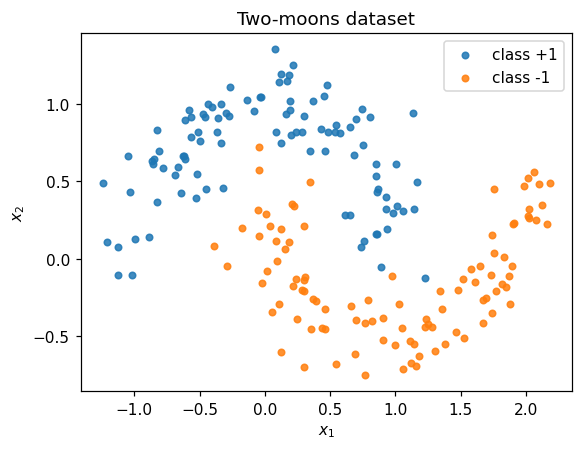
\includegraphics[width=0.58\textwidth]{figures/dataset.png}
\caption{The two-moons dataset: 200 samples with Gaussian noise
($\sigma = 0.15$), labels in $\{-1,+1\}$.}
\label{fig:data}
\end{figure}

\begin{figure}[h]
\centering
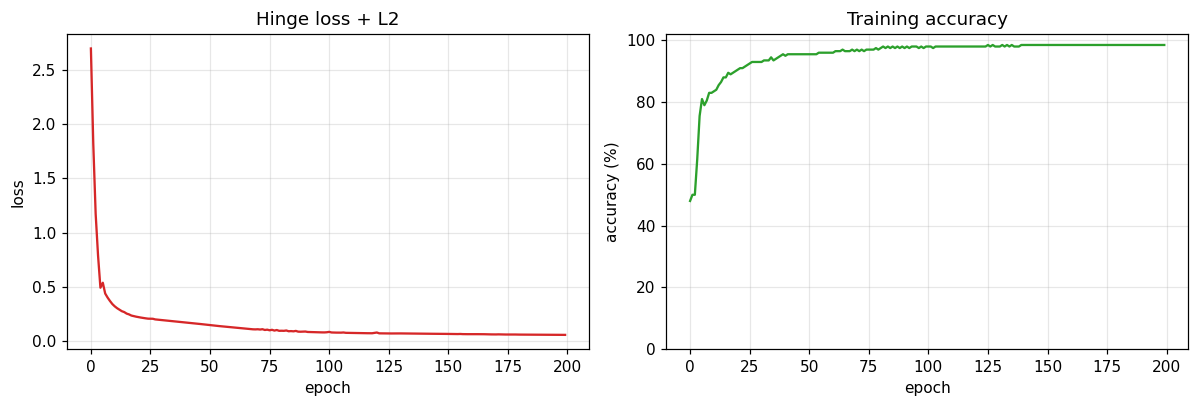
\includegraphics[width=0.92\textwidth]{figures/learning_curves.png}
\caption{Left: mean hinge loss $+$ L2 over training. Right: training
accuracy. Both improve monotonically under full-batch SGD with learning-rate
decay.}
\label{fig:curves}
\end{figure}

\begin{figure}[h]
\centering
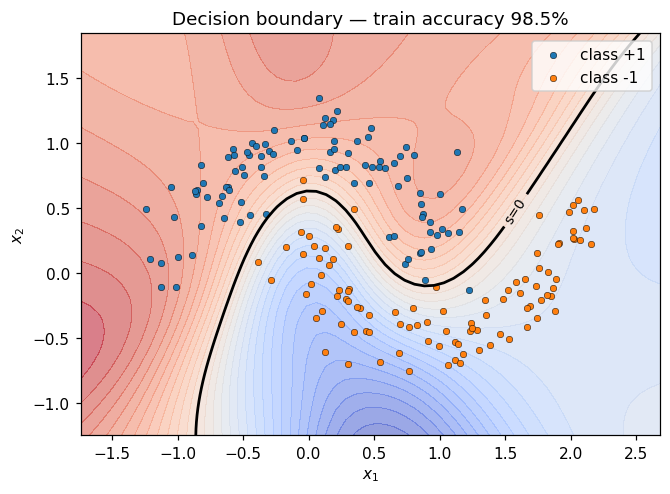
\includegraphics[width=0.62\textwidth]{figures/decision_boundary.png}
\caption{Decision boundary of the trained network (score $s(x)=0$ contour) and
the training points.}
\label{fig:boundary}
\end{figure}

Loss falls monotonically from $2.70$ to $0.0597$ while training accuracy rises
from $48\%$ (random) to \textbf{98.5\%} (Figure~\ref{fig:curves}); the decision
boundary in Figure~\ref{fig:boundary} follows the two arcs closely, correctly
separating the interleaved crescents. The loss keeps decreasing after
accuracy saturates because the hinge loss continues to widen the margin on the
few remaining ambiguous points.

\section{Answers to the conceptual questions}
\label{sec:questions}

The template repository does not list explicit questions; the set below covers
the concepts the plan and assignment description emphasise (chain rule,
reverse mode, topological sorting, diamonds, design choices, NN API). If the
LMS publishes additional questions, they should be appended here.

\begin{enumerate}
  \item \textbf{Why does the gradient flow from the output to the inputs?}
  Because $L$ is a composition of local functions; Eq.~\eqref{eq:chain} is a
  recursion from $L$ downwards. Seeding $\partial L/\partial L = 1$ and
  visiting nodes in reverse topological order evaluates that recursion once,
  giving every parameter's gradient in a single $\mathcal{O}(|V|)$ sweep.

  \item \textbf{Why is a topological sort needed, and why post-order?}
  A node may only be backpropagated through after all consumers of its
  gradient have contributed (otherwise it pushes an incomplete gradient).
  Post-order DFS lists every node after its dependencies; reversing that list
  yields a valid processing order starting from the output.

  \item \textbf{Why the \texttt{visited} set?}
  DAGs share nodes. Without it, a shared node is visited once per path
  (exponential in depth) and would be appended multiple times to the topo
  list, causing its outgoing gradient to be applied several times ---
  double-counted gradients. See Section~\ref{sec:diamond}.

  \item \textbf{Why must local backward rules use \texttt{+=}?}
  Because a node can receive gradient from several parents (and from several
  operands of the same operation, as in $a+a$); Eq.~\eqref{eq:chain} is a
  \emph{sum} over paths. Assignment would let the last path overwrite the
  earlier ones: for $d=(a+a)\cdot a$ we would obtain $3$ instead of $12$.

  \item \textbf{Why seed the root's gradient with $1.0$?}
  We differentiate $L$ with respect to itself, $\partial L/\partial L = 1$;
  everything else follows by the chain rule. It also means an intermediate
  node used as the seed yields the gradient of \emph{that node} w.r.t.\ the
  inputs, which is what makes intermediate-value tests possible.

  \item \textbf{What would change for a vector-valued output?}
  Reverse-mode gives one output's gradient per sweep; a Jacobian with $m$
  outputs requires $m$ backward passes (or a framework with vector-Jacobian
  products). Deep learning keeps a scalar loss precisely so one pass suffices.

  \item \textbf{Why is \texttt{pow} restricted to constant exponents?}
  $\partial_a a^{k} = k a^{k-1}$ holds only for constant $k$; a
  \texttt{Value} exponent would add $a^{k}\ln a \cdot \partial k/\partial a$,
  which the local rule does not implement. An assertion fails fast instead of
  returning a silently wrong gradient.

  \item \textbf{Why uniform weights in $[-1,1]$?}
  Keeps initial pre-activations in \texttt{tanh}'s linear region
  ($1-\tanh^{2} \approx 1$) so every unit can learn from step 1; symmetric
  random values also break unit symmetry. See Section~\ref{sec:design}.

  \item \textbf{Why \texttt{tanh} instead of sigmoid?}
  Zero-centred outputs ($(-1,1)$) give better-conditioned gradients for
  downstream layers, while remaining smooth and bounded; the derivative
  $1-t^{2}$ reuses the forward value. The output layer stays linear so scores
  are not clipped by the margin loss.

  \item \textbf{How does this compare to PyTorch?}
  PyTorch executes the same two-phase protocol (record graph in forward,
  walk it in reverse) but on tensors with fused C++/CUDA kernels, a dynamic
  autograd graph per iteration, and \texttt{Tensor.grad} accumulation that is
  semantically identical to our \texttt{+=}. Our \texttt{Value} is the scalar
  special case of a \texttt{Tensor}.

  \item \textbf{Why is NumPy/PyTorch not allowed here?}
  The point of the exercise is to internalise the mechanics --- computational
  graphs, local derivatives, topological ordering, accumulation --- rather
  than to obtain gradients from a library. NumPy is used in the notebook only
  for dataset generation and plotting, never inside \texttt{engine.py} /
  \texttt{nn.py}.
\end{enumerate}

\section{Reproducibility}

\begin{verbatim}
python -m pytest            # 42 tests, from the repository root
jupyter nbconvert --to notebook --execute demo.ipynb   # or Restart & Run All
cd report && tectonic main.tex                          # this PDF
\end{verbatim}

No PyTorch (or any autodiff library) is imported by \texttt{src/engine.py} or
\texttt{src/nn.py}; the engine depends only on the standard-library
\texttt{math} module.

\end{document}
